\documentclass[a4paper,11pt]{article}

\pdfminorversion=4

\usepackage{cmap}
\usepackage[utf8]{inputenc}
\usepackage[T1]{fontenc}
\usepackage{lmodern}
\usepackage{geometry}
\usepackage{graphicx}
\usepackage{amsmath}
\usepackage{amssymb}
\usepackage{xcolor}
\usepackage{listings}
\usepackage{float}
\usepackage{hyperref}

\geometry{margin=2.4cm}
\setlength{\parindent}{0pt}
\setlength{\parskip}{0.65em}
\setlength{\emergencystretch}{2em}
\renewcommand{\abstractname}{Resumo}
\renewcommand{\figurename}{Figura}

\lstset{
  basicstyle=\ttfamily\small,
  breaklines=true,
  frame=none,
  backgroundcolor=\color{gray!8},
  xleftmargin=1em,
  xrightmargin=1em,
}

\title{Arquitetura de Software como Representa\c{c}\~ao em Camadas\\
  \large An\'alise de Arquitetura de Software com S202}
\author{Johannes Weigend}
\date{Vers\~ao final, 26~de maio de~2026}

\begin{document}

\maketitle

\begin{abstract}
S202 calcula, a partir de bytecode, uma representa\c{c}\~ao hier\'arquica em
camadas de sistemas Java. A ferramenta deriva uma hip\'otese arquitetural das
depend\^encias observadas entre classes, torna ciclos e back edges vis\'iveis
como achados expl\'icitos e verifica a representa\c{c}\~ao final de forma
redundante contra regras de consist\^encia. Este documento descreve erros
t\'ipicos no c\'alculo desses layouts, explica a solu\c{c}\~ao conceitual e
mostra como a representa\c{c}\~ao pode ser usada como ferramenta de trabalho
para planejamento de refatora\c{c}\~ao.
\end{abstract}

\section{Introdu\c{c}\~ao}

Pelo menos desde os modelos em camadas para sistemas operacionais no fim da
d\'ecada de 1960, a arquitetura de software vem sendo representada como uma
estrutura de depend\^encias em camadas. Esse princ\'ipio continua atual: em
arquiteturas cloud native ele ajuda a ordenar depend\^encias t\'ecnicas entre
servi\c{c}os, plataformas e infraestrutura; no domain-driven design, ajuda a
tornar vis\'iveis os limites de dom\'inio e as depend\^encias entre bounded
contexts. A ideia b\'asica \'e simples: um elemento que usa outro elemento
fica acima do elemento usado. As depend\^encias, portanto, correm de cima para
baixo. Arestas na dire\c{c}\~ao oposta chamam a aten\c{c}\~ao porque muitas
vezes indicam ciclos, acoplamento indesejado ou uma ordem em camadas
quebrada.

Grafos alinhados verticalmente desse tipo ajudam a entender sistemas e a
reconhecer anomalias em suas depend\^encias. Um exemplo simples \'e fornecido
pela ferramenta Java \texttt{jdeps} e pela ferramenta Graphviz \texttt{dot}:
\texttt{jdeps} extrai as depend\^encias entre classes de um JAR, e
\texttt{dot} gera a partir delas um grafo dirigido.

\newpage

A Figura~\ref{fig:acyclic-levels} mostra um exemplo ac\'iclico do Example JAR
da base de c\'odigo do S202. Ele foi criado com \texttt{jdeps} e \texttt{dot}.
O JAR cont\'em nove classes em tr\^es pacotes: \texttt{example},
\texttt{example1} e \texttt{example2}.

\begin{figure}[H]
  \centering
  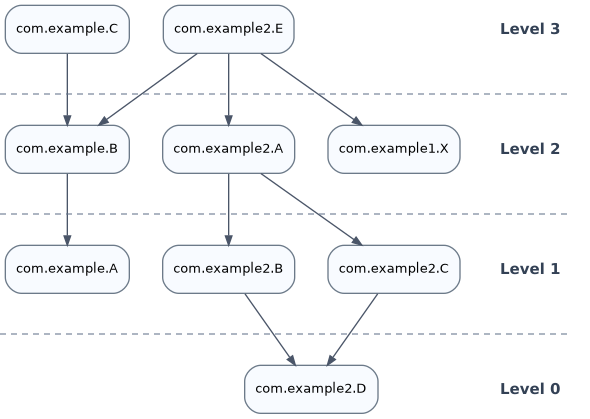
\includegraphics[width=0.75\textwidth]{figures/test-example-classgraph-acyclic-levels.png}
  \caption{Exemplo ac\'iclico de \texttt{test-example-1.0.0.jar}.}
  \label{fig:acyclic-levels}
\end{figure}

As setas entre as caixas s\~ao depend\^encias entre classes por chamada ou uso.
No exemplo, \texttt{com.example.B} usa a classe \texttt{com.example.A}, de
forma abreviada $B \to A$. As linhas horizontais foram acrescentadas
manualmente e visualizam os n\'iveis da camada. O Level~0 forma a base;
n\'iveis mais altos representam elementos que dependem de elementos abaixo
deles.

Esse tipo de representa\c{c}\~ao \'e \'util e amplamente usado. Como
visualiza\c{c}\~ao de aplica\c{c}\~oes reais, por\'em, ele tem tr\^es
problemas pr\'aticos:

\begin{enumerate}
  \item Muitas setas tornam o grafo confuso j\'a em aplica\c{c}\~oes de porte
        m\'edio.
  \item A estrutura de pacotes fica distribu\'ida por v\'arios n\'iveis e n\~ao
        forma um agrupamento vis\'ivel.
  \item Em depend\^encias c\'iclicas, o ciclo precisa ser quebrado para o
        c\'alculo dos n\'iveis, para que surja alguma ordem vertical. O grafo
        original de depend\^encias permanece inalterado; muda apenas o DAG
        derivado (\emph{Directed Acyclic Graph}, um grafo dirigido sem ciclos)
        sobre o qual os n\'iveis s\~ao calculados. A quest\~ao decisiva,
        portanto, \'e qual aresta fica fora desse c\'alculo, pois exatamente
        essa aresta aparece depois como quebra da ordem calculada.
\end{enumerate}

\section{S202 como Representa\c{c}\~ao Hier\'arquica em Camadas}

Com a ferramenta open source S202, buscamos tratar esses problemas de forma
direta. S202 n\~ao substitui simplesmente o grafo plano de classes por uma
representa\c{c}\~ao melhorada. Ele o substitui por uma hip\'otese arquitetural
hier\'arquica: pacotes permanecem vis\'iveis como cont\^eineres e, dentro de
cada cont\^einer, pacotes ou classes s\~ao ordenados de acordo com suas
depend\^encias.

As setas podem ser exibidas opcionalmente. Normalmente, por\'em, a ordem
vertical j\'a deve deixar compreens\'ivel quais partes da aplica\c{c}\~ao
ficam mais acima e quais servem de base. Depend\^encias indesejadas, assim,
n\~ao aparecem apenas como uma linha isolada em uma grande rede, mas como uma
quebra em uma ordem esperada de camadas.

Ao contr\'ario do grafo plano de classes, em S202 os n\'iveis s\~ao
estruturados hierarquicamente pela estrutura de pacotes. Cada pacote ordena
seus filhos diretos, isto \'e, subpacotes ou classes, segundo suas
depend\^encias locais. A estrutura de pacotes permanece vis\'ivel, em vez de
ser espalhada pelo grafo de classes.

\begin{figure}[H]
  \centering
  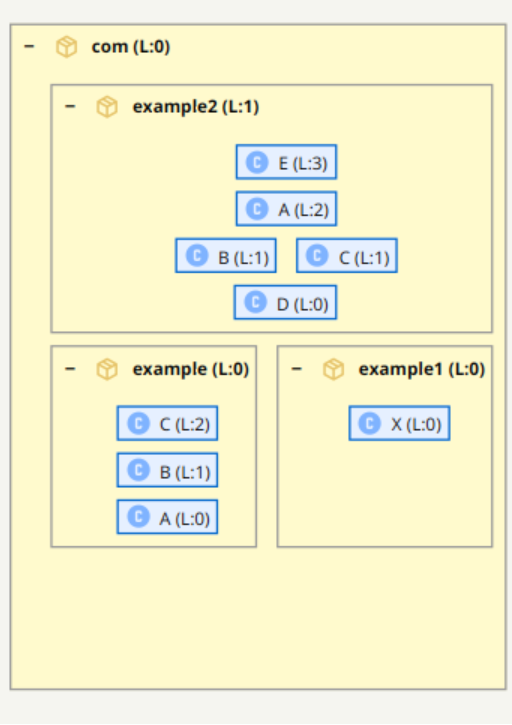
\includegraphics[width=0.55\textwidth]{figures/s202-dependencies-acyclic.png}
  \caption{Representa\c{c}\~ao S202 do exemplo ac\'iclico: pacotes permanecem
  vis\'iveis como cont\^eineres, classes s\~ao ordenadas dentro de seu
  cont\^einer e setas podem ser exibidas quando necess\'ario.}
  \label{fig:s202-acyclic}
\end{figure}

O exemplo mostra a estrutura de pacotes abaixo do pacote externo
\texttt{com}: \texttt{example}, \texttt{example1} e \texttt{example2} s\~ao
sub\'arvores desse cont\^einer. Na sub\'arvore \texttt{example2} existe uma
estrutura interna de classes n\~ao trivial; ao mesmo tempo, a estrutura mais
ampla mostra que \texttt{example2} depende de \texttt{example} e
\texttt{example1}. No n\'ivel de classes vale, para \texttt{example2},
$E \to A \to (B \mid C) \to D$. A representa\c{c}\~ao abstrai
deliberadamente das arestas individuais. Se \texttt{A} tem uma depend\^encia
para \texttt{B}, para \texttt{C} ou para ambos \'e menos importante para a
vis\~ao arquitetural ampla do que a estrutura em camadas do pacote. Exatamente
essa abstra\c{c}\~ao torna redes extensas de rela\c{c}\~oes ainda leg\'iveis.

A ideia n\~ao \'e nova. O produto comercial Structure101 j\'a tinha uma
representa\c{c}\~ao muito semelhante. No entanto, n\~ao h\'a uma
implementa\c{c}\~ao aberta nem uma documenta\c{c}\~ao t\'ecnica que explique
como calcular esse layout de forma confi\'avel. S202 fecha essa lacuna como
ferramenta open source sob a licen\c{c}a Apache.

Este documento descreve as armadilhas t\'ipicas na realiza\c{c}\~ao de um
layout desse tipo e mostra uma solu\c{c}\~ao com a qual muitos desses
problemas podem ser eliminados de forma conceitualmente limpa.

\section{Erros T\'ipicos no C\'alculo de Camadas}

As Figuras~\ref{fig:acyclic-levels} e~\ref{fig:s202-acyclic} mostram
deliberadamente um exemplo simples e ac\'iclico. Nesse caso, a camada \'e
inequ\'ivoca: \texttt{E} fica acima de \texttt{A}, \texttt{A} fica acima de
\texttt{B} e \texttt{C}, e ambos ficam acima de \texttt{D}. N\~ao h\'a
realimenta\c{c}\~ao, portanto nenhuma aresta precisa ser escolhida para ser
ignorada no c\'alculo dos n\'iveis.

Em aplica\c{c}\~oes reais esse caso \'e mais exce\c{c}\~ao do que regra. Assim
que classes ou pacotes dependem ciclicamente uns dos outros, uma passagem
normal pelo grafo n\~ao basta mais. \'E exatamente a\'i que come\c{c}am os
erros interessantes: a representa\c{c}\~ao muitas vezes ainda parece
plaus\'ivel, mas os n\'iveis calculados deixam de ser est\'aveis ou deixam de
ser explic\'aveis em termos arquiteturais.

Nas se\c{c}\~oes seguintes, o termo SCC tem papel central. Uma SCC
(\emph{Strongly Connected Component}, componente fortemente conexa) \'e um
conjunto de n\'os no qual cada n\'o pode alcan\c{c}ar todos os outros por
caminhos dirigidos de depend\^encia. Em um ciclo desse tipo, nem todas as
depend\^encias podem correr para baixo ao mesmo tempo.

Um layout em camadas correto precisa, portanto, satisfazer v\'arios requisitos
ao mesmo tempo:

\begin{enumerate}
  \item Se $A \to B$, ent\~ao $A$ deve ficar acima de $B$.
  \item Pacotes precisam permanecer vis\'iveis como cont\^eineres. Um pacote
        n\~ao deve ser deslocado por acaso apenas porque uma classe contida
        nele tem um n\'ivel de classe alto.
  \item Classes ou pacotes que formam uma SCC precisam ser tratados
        explicitamente, porque em um ciclo nem todas as arestas podem correr
        para baixo ao mesmo tempo.
\end{enumerate}

Esses requisitos s\~ao individualmente bem resolv\'iveis. Juntos, por\'em,
eles criam um sistema circular de depend\^encias entre os pr\'oprios n\'iveis
da computa\c{c}\~ao: n\'iveis de classes influenciam posi\c{c}\~oes
vis\'iveis, cont\^eineres de pacotes estruturam essas posi\c{c}\~oes, e SCCs
for\c{c}am corre\c{c}\~oes em uma ordem que j\'a teria sido calculada sem o
tratamento de ciclos. \'E da\'i que surgem os modos t\'ipicos de falha.

\subsection{Corre\c{c}\~ao Retroativa}

Corre\c{c}\~ao retroativa significa aqui: uma estrutura reconhecida mais tarde
obriga uma altera\c{c}\~ao posterior em n\'iveis j\'a calculados.

Um algoritmo ing\^enuo percorre as classes e atribui n\'iveis diretamente. Ele
v\^e primeiro a classe \texttt{A}, define seu n\'ivel e com isso tamb\'em
eleva o pacote de \texttt{A}. Mais tarde encontra a classe \texttt{B} e
reconhece: \texttt{A} e \texttt{B} pertencem \`a mesma SCC e precisam ser
tratadas em conjunto. Agora \texttt{A} teria de ser corrigida, e com ela seu
pacote e possivelmente outros pacotes que dependem dele.

O problema n\~ao \'e a corre\c{c}\~ao em si. O problema \'e que partes do
layout, nesse momento, j\'a foram tratadas como conclu\'idas. Um algoritmo que
mistura detec\c{c}\~ao de ciclos e atribui\c{c}\~ao de n\'iveis precisa
alterar retroativamente lugares que ele na verdade j\'a deixou para tr\'as.

\subsection{Resultados Dependentes da Ordem}

Classes v\^em de JARs. A ordem em que uma ferramenta v\^e classes n\~ao segue
a arquitetura, mas a ordem de empacotamento do JAR, a ordem dos m\'odulos, a
ferramenta de build ou detalhes do sistema de arquivos. Se um algoritmo trata
ciclos incidentalmente durante essa travessia, o resultado depende dessa ordem
acidental.

Isso \'e perigoso porque o erro n\~ao precisa ser vis\'ivel imediatamente. O
grafo ainda pode parecer aproximadamente correto. Mesmo assim, a mesma base de
c\'odigo pode receber n\'iveis diferentes dependendo da configura\c{c}\~ao de
build.

\subsection{Mistura de N\'iveis de Classe e de Pacote}

Um erro natural \'e derivar o n\'ivel de um pacote a partir do maior n\'ivel de
suas classes contidas. Isso parece plaus\'ivel, mas mistura duas perguntas
diferentes: onde uma classe fica no grafo de classes e onde um pacote fica na
hip\'otese arquitetural.

Um pacote n\~ao est\'a arquiteturalmente alto apenas porque por acaso cont\'em
uma classe posicionada alto. A regra central \'e:

\begin{quote}
  N\'iveis de pacotes surgem de depend\^encias entre pacotes, n\~ao da altura
  m\'axima de classes individuais.
\end{quote}

Isso parece trivial, mas n\~ao \'e. Justamente porque pacotes s\~ao
cont\^eineres de classes, parece natural derivar sua posi\c{c}\~ao das classes
contidas. Mas \'e exatamente assim que se misturam dois n\'iveis que precisam
permanecer separados. Somente quando n\'iveis de pacotes surgem de
depend\^encias entre pacotes, os pacotes permanecem unidades arquiteturais
est\'aveis. Caso contr\'ario, uma \'unica classe fora do padr\~ao basta para
elevar o pacote ao n\'ivel errado e tornar inutiliz\'avel o cont\^einer que
deveria oferecer orienta\c{c}\~ao.

\subsection{O Grande Lago}

A resposta formalmente limpa para ciclos \'e: todos os elementos de uma SCC
recebem o mesmo n\'ivel. Para ciclos pequenos isso \'e aceit\'avel. Em sistemas
reais, por\'em, SCCs podem ficar muito grandes. Ent\~ao centenas ou milhares
de classes acabam no mesmo n\'ivel. A camada desaparece; o que resta \'e um
bloco plano.

O ciclo, assim, foi reconhecido corretamente, mas deixou de ser visualizado de
forma \'util. Uma ferramenta precisa, portanto, conseguir quebrar SCCs grandes.
O ponto decisivo \'e que as arestas cortadas n\~ao podem desaparecer. Elas
precisam permanecer vis\'iveis, porque explicam por que a ordem calculada vale
apenas como hip\'otese arquitetural.

\section{O Grafo de Pacotes como Hip\'otese Arquitetural}

A solu\c{c}\~ao escolhida pelo S202 consiste em separar de forma consequente a
an\'alise, a forma\c{c}\~ao da ordem e a representa\c{c}\~ao. O grafo de
classes permanece o modelo bruto das depend\^encias reais. Ele n\~ao \'e
alterado apenas porque uma representa\c{c}\~ao em camadas precisa de um DAG.
Em vez disso, S202 cria a partir desse grafo vis\~oes adicionais: SCCs para a
detec\c{c}\~ao de ciclos, um grafo de pacotes ponderado para a hip\'otese
arquitetural e uma estrutura hier\'arquica de UI para a representa\c{c}\~ao.

Com hip\'otese arquitetural n\~ao se quer dizer uma arquitetura-alvo afirmada.
Quer-se dizer uma arquitetura real inferida das depend\^encias observadas: a
ordem que melhor corresponde ao c\'odigo existente e a suas depend\^encias sem
esconder onde essa ordem \'e quebrada por ciclos ou back edges.

A ordem de pacotes forma o elo central. Ela n\~ao \'e derivada dos maiores
n\'iveis de classes, mas das depend\^encias agregadas entre pacotes. Essa
separa\c{c}\~ao \'e o passo decisivo: classes s\~ao ordenadas dentro de seus
pacotes; pacotes, por sua vez, s\~ao ordenados por suas pr\'oprias
rela\c{c}\~oes entre pacotes. Assim, um pacote pode permanecer est\'avel como
cont\^einer, mesmo que classes individuais dentro dele fiquem altas ou baixas.
Ao mesmo tempo, a ordem de pacotes fornece um crit\'erio para escolher back
edges n\~ao arbitrariamente, mas como viola\c{c}\~oes concretas da ordem
esperada.

Com isso, os modos de falha descritos acima n\~ao desaparecem por meio de um
truque algor\'itmico isolado, mas por uma responsabilidade clara das etapas de
c\'alculo: primeiro as depend\^encias s\~ao analisadas, depois uma ordem
plaus\'ivel \'e determinada, em seguida a estrutura vis\'ivel \'e constru\'ida
e, por fim, verifica-se se a representa\c{c}\~ao cumpre sua pr\'opria
afirma\c{c}\~ao.

\section{De Depend\^encias de Classes \`a Ordem de Pacotes}

O grafo plano de classes n\~ao \'e, em S202, o modelo vis\'ivel de layout. Ele
\'e um artefato de an\'alise: serve para registrar depend\^encias concretas,
reconhecer SCCs, agregar depend\^encias de classes em rela\c{c}\~oes entre
pacotes e derivar delas os n\'iveis posteriores. A representa\c{c}\~ao S202
vis\'ivel surge depois da estrutura de pacotes e da ordem local dentro dos
cont\^eineres de pacotes.

A ordem de pacotes surge localmente no contexto de um pacote pai. S202 n\~ao
compara pacotes arbitr\'arios globalmente; compara sempre os pacotes filhos
diretos do mesmo cont\^einer. Classes n\~ao s\~ao n\'os de compara\c{c}\~ao
nessa etapa. Elas fornecem a informa\c{c}\~ao para a agrega\c{c}\~ao: uma
depend\^encia de classe \'e elevada aos pacotes filhos em cujas sub\'arvores
est\~ao a origem e o destino.

Para cada pacote pai surge assim um grafo ponderado de irm\~aos de seus
pacotes filhos. As arestas nesse grafo s\~ao depend\^encias de pacotes
observadas diretamente entre esses pacotes filhos. Se uma classe na
sub\'arvore do pacote filho $P$ usa uma classe na sub\'arvore do pacote filho
$Q$, surge uma aresta $P \to Q$. Seu peso \'e a quantidade de usos concretos
elevados para essa aresta de pacote; para depend\^encias estruturais sem
contagem de chamadas, usa-se peso~1. A dire\c{c}\~ao contr\'aria tamb\'em \'e
contada.

O grafo de irm\~aos cont\'em apenas essas depend\^encias diretas entre
pacotes. De $B \to A$ e $C \to B$ n\~ao se cria uma aresta adicional
$C \to A$. A ordem transitiva surge apenas no c\'alculo posterior dos
n\'iveis. Depend\^encias dentro do mesmo pacote filho n\~ao alteram a ordem dos
pacotes filhos; depend\^encias que saem do cont\^einer pai s\~ao tratadas em
um n\'ivel mais alto da estrutura de pacotes. Essa compara\c{c}\~ao \'e
repetida recursivamente para todos os cont\^eineres de pacotes. A ordem das
classes dentro de um cont\^einer de pacote \'e uma etapa posterior.

Antes do c\'alculo dos n\'iveis, o grafo de irm\~aos precisa ser ac\'iclico. Se
pacotes filhos formam uma SCC, S202 usa uma medida de rank para avaliar se um
pacote filho, no grafo de irm\~aos atual, tende mais a usar outros pacotes ou
a ser usado por eles:

\[
  rank(P) = \frac{out(P) - in(P)}{\max(1,\; out(P) + in(P))}
\]

$out(P)$ \'e a soma dos pesos das arestas de $P$ para outros irm\~aos
considerados no grafo atual, e $in(P)$ \'e a soma dos pesos das arestas desses
irm\~aos para $P$. Um rank positivo significa: o pacote usa mais do que ele
mesmo \'e usado; ele tende a pertencer mais acima. Um rank negativo significa:
o pacote \'e mais usado e tende a pertencer mais abaixo.

Em uma SCC de pacotes, uma aresta $P \to Q$ s\'o \'e tratada como back edge
quando $rank(P)$ fica abaixo de $rank(Q)$ por mais que uma toler\^ancia
$\varepsilon$. Atualmente, S202 usa $\varepsilon = 0{,}1$ para isso. Se dois
pacotes ficam pr\'oximos demais, eles permanecem conceitualmente como pares e
portanto no mesmo n\'ivel. Uma rela\c{c}\~ao rec\'iproca de chamadas de
$100 : 101$ n\~ao \'e, por isso, uma decis\~ao arquitetural robusta.

Depois desse tratamento de ciclos, S202 calcula os n\'iveis sobre o DAG
resultante. O Level~0 cont\'em os pacotes que, no grafo de c\'alculo atual,
n\~ao usam nenhum outro pacote filho. Todo outro pacote fica um n\'ivel acima
do pacote mais alto que ele usa diretamente. Assim surge a estratifica\c{c}\~ao
transitiva: de $B \to A$ e $C \to B$ segue que $A$ fica no Level~0, $B$ no
Level~1 e $C$ no Level~2, mesmo sem existir uma aresta direta $C \to A$.

\section{Do Ciclo de Classes \`a Ordem de Pacotes}

A Figura~\ref{fig:cyclic-class} mostra um exemplo c\'iclico do Example JAR
como grafo cl\'assico de classes. Os dois subgrafos para Notification e
Payment cont\^em realimenta\c{c}\~oes.

\begin{figure}[H]
  \centering
  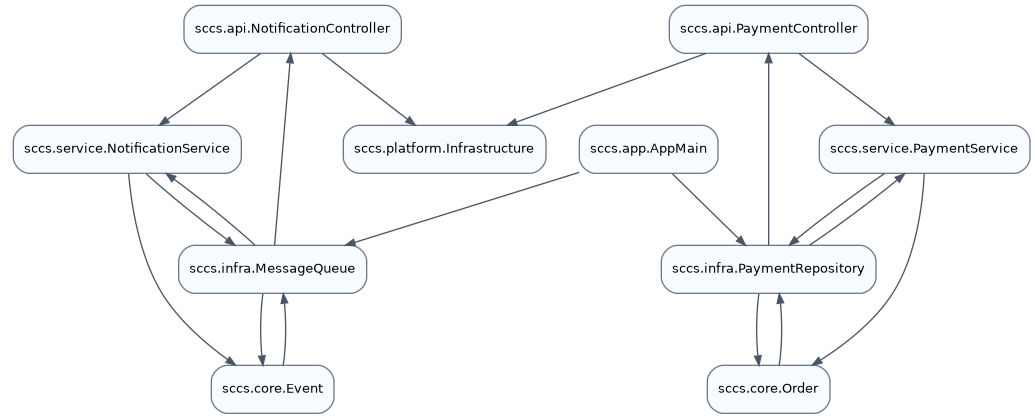
\includegraphics[width=0.9\textwidth]{figures/test-example-classgraph-cyclic.png}
  \caption{Exemplo c\'iclico de \texttt{test-example-1.0.0.jar}. Em cada ciclo,
  pelo menos uma aresta precisa ser cortada para o c\'alculo dos n\'iveis.}
  \label{fig:cyclic-class}
\end{figure}

As regi\~oes c\'iclicas marcadas s\~ao duas SCCs n\~ao triviais: uma SCC de
Notification com \texttt{NotificationController},
\texttt{NotificationService}, \texttt{MessageQueue} e \texttt{Event}, e uma
SCC de Payment com \texttt{PaymentController}, \texttt{PaymentService},
\texttt{PaymentRepository} e \texttt{Order}. O procedimento estabelecido para
encontrar esses componentes \'e o algoritmo de Tarjan.

No caso c\'iclico, o grafo de classes coloca a pergunta t\'ecnica: qual aresta
precisa ser ignorada para que a SCC volte a ser um DAG calcul\'avel para a
forma\c{c}\~ao dos n\'iveis? Mas o grafo de classes sozinho n\~ao fornece um
crit\'erio arquitetural para isso. Somente a ordem de pacotes fornece esse
crit\'erio: uma aresta classificada como back edge n\~ao \'e ent\~ao uma aresta
de corte arbitr\'aria no grafo plano de classes, mas uma depend\^encia concreta
que corre contra a ordem de pacotes calculada e, assim, torna vis\'ivel a
quebra na hip\'otese arquitetural.

\begin{figure}[H]
  \centering
  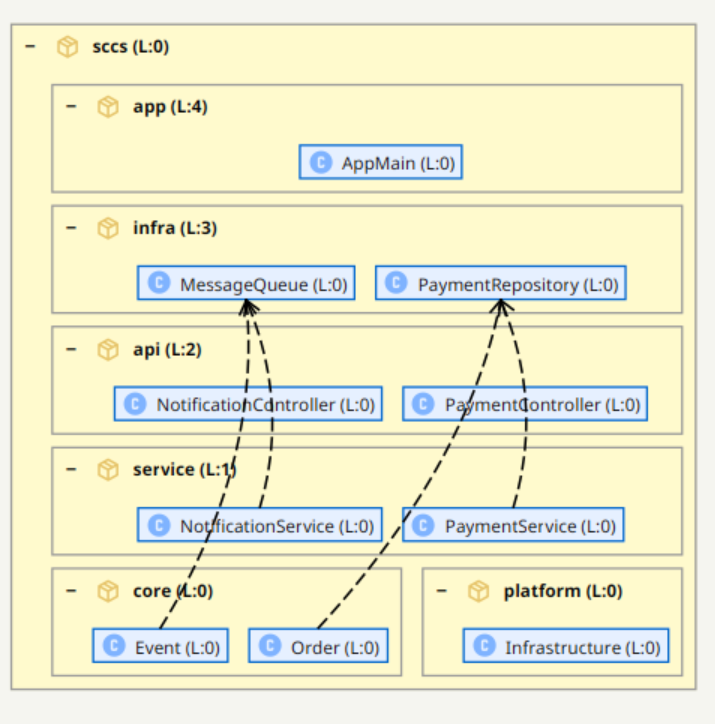
\includegraphics[width=0.6\textwidth]{figures/s202-dependencies-cyclic.png}
  \caption{Exemplo c\'iclico na representa\c{c}\~ao S202. As arestas tracejadas
  s\~ao viola\c{c}\~oes: elas correm contra a ordem derivada das depend\^encias
  entre pacotes e permanecem como achados vis\'iveis da hip\'otese
  arquitetural. Todas as quatro arestas tracejadas pertencem \`as duas SCCs e
  s\~ao classificadas pelo S202 como back edges para o c\'alculo dos n\'iveis.}
  \label{fig:s202-cyclic}
\end{figure}

Os termos back edge e viola\c{c}\~ao descrevem pap\'eis diferentes:

\begin{description}
  \item[Back edge] Uma aresta escolhida dentro de uma SCC que \'e tratada
        separadamente no c\'alculo dos n\'iveis para que o grafo de c\'alculo
        se torne ac\'iclico. Ela pertence ao tratamento de ciclos.
  \item[Viola\c{c}\~ao] Uma depend\^encia concreta que, depois da ordem
        calculada, corre para cima. Ela pode vir de uma SCC, mas n\~ao precisa.
        Viola\c{c}\~oes s\~ao portanto um superconjunto dos back edges: um
        back edge pode tornar-se vis\'ivel como viola\c{c}\~ao, mas nem toda
        viola\c{c}\~ao \'e um back edge. Conceitualmente, a viola\c{c}\~ao
        continua sendo o desvio vis\'ivel da ordem, enquanto um back edge
        descreve o papel da aresta no tratamento de ciclos.
\end{description}

S202, portanto, n\~ao esconde o ciclo. Arestas classificadas como back edges
permanecem vis\'iveis como viola\c{c}\~oes porque explicam por que a ordem de
pacotes n\~ao corresponde completamente \`as depend\^encias concretas entre
classes. Assim, o desvio se torna rastre\'avel em vez de arbitr\'ario.

\section{Verifica\c{c}\~ao Redundante da Consist\^encia}

As etapas descritas at\'e aqui j\'a mostram por que a implementa\c{c}\~ao \'e
propensa a erros. N\~ao basta proteger algoritmos isolados com unit tests.
Muitos erros surgem apenas da intera\c{c}\~ao dos dados: depend\^encias
concretas entre classes, estrutura de pacotes, SCCs, pesos agregados de
pacotes e posi\c{c}\~oes locais de representa\c{c}\~ao influenciam-se
mutuamente.

Por isso S202 n\~ao verifica apenas passos individuais de c\'alculo. Depois
que toda a pipeline rodou, o resultado final \'e verificado de forma
redundante contra regras de consist\^encia. Essas regras n\~ao recalculam o
layout e n\~ao corrigem nada. Elas apenas leem o resultado e perguntam: a
representa\c{c}\~ao gerada \'e consistente em si mesma?

A verifica\c{c}\~ao considera tr\^es n\'iveis:

\begin{enumerate}
  \item \textbf{Grafo de classes:} Para depend\^encias normais entre classes
        deve valer: se $A \to B$, ent\~ao $A$ est\'a em um n\'ivel mais alto
        que $B$. Exce\c{c}\~oes precisam ser classificadas explicitamente, por
        exemplo como back edge ou como aresta dentro de uma SCC.
  \item \textbf{Grafo de pacotes:} A ordem de pacotes calculada precisa
        combinar com as depend\^encias ponderadas entre pacotes. Pacotes com
        rank mais alto precisam ficar acima dos pacotes dos quais dependem com
        mais for\c{c}a. Arestas cortadas ao quebrar uma SCC de pacotes n\~ao
        podem ser tratadas nessa verifica\c{c}\~ao como arestas dominantes
        normais; elas precisam ser classificadas separadamente como back edges
        de pacotes.
  \item \textbf{Representa\c{c}\~ao vis\'ivel:} A disposi\c{c}\~ao vis\'ivel
        precisa corresponder ao modelo calculado. Cont\^eineres de pacotes,
        posi\c{c}\~oes locais de classes e n\'iveis aninhados n\~ao podem
        inverter silenciosamente a hip\'otese arquitetural calculada.
\end{enumerate}

Essas regras de consist\^encia n\~ao s\~ao uma otimiza\c{c}\~ao adicional nem
um segundo algoritmo de layout. Elas s\~ao uma verifica\c{c}\~ao independente
de plausibilidade ap\'os o fim do c\'alculo. Exatamente por isso encontram
erros que faltam facilmente em unit tests normais: um n\'ivel de pacote foi
calculado corretamente, mas exibido localmente de forma errada; um back edge
foi cortado, mas n\~ao marcado como tal; uma aresta normal corre para cima sem
ser parte de uma SCC.

O ponto decisivo \'e a redund\^ancia. A pipeline gera a representa\c{c}\~ao. As
regras verificam em seguida se essa representa\c{c}\~ao cumpre sua pr\'opria
afirma\c{c}\~ao. Com isso, uma simples figura se torna um modelo verific\'avel.

\section{Da Visualiza\c{c}\~ao \`a A\c{c}\~ao}

Uma hip\'otese arquitetural calculada \'e especialmente \'util quando n\~ao
apenas descreve um estado, mas torna mudan\c{c}as planej\'aveis. Para isso,
S202 cont\'em uma an\'alise what-if: classes e pacotes podem ser movidos por
drag and drop na representa\c{c}\~ao. O modelo n\~ao \'e refatorado
imediatamente; em vez disso, a ferramenta calcula quais depend\^encias
passariam a correr para cima na nova disposi\c{c}\~ao.

As viola\c{c}\~oes se atualizam ap\'os cada deslocamento. Assim fica vis\'ivel
se uma reordena\c{c}\~ao planejada torna a arquitetura mais consistente ou
cria novos problemas. Isso \'e importante sobretudo em situa\c{c}\~oes nas
quais a ferramenta n\~ao encontra mais uma ordem inequ\'ivoca: SCCs grandes,
depend\^encias sim\'etricas entre pacotes ou acoplamentos historicamente
crescidos nem sempre podem ser resolvidos automaticamente de maneira sensata.

\begin{figure}[H]
  \centering
  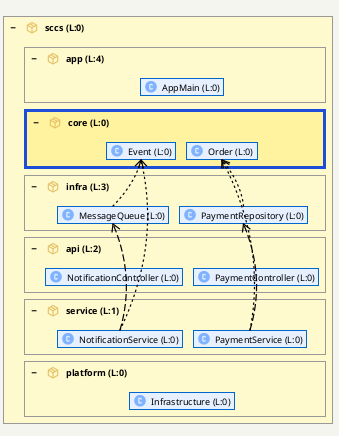
\includegraphics[width=0.45\textwidth]{figures/whatif-core-over-infra.png}
  \caption{Movimento what-if: o pacote \texttt{core} \'e movido do Level~0 para
  entre o Level~3 e o Level~4. Isso cria seis viola\c{c}\~oes, porque
  depend\^encias existentes agora correm contra a disposi\c{c}\~ao escolhida.}
  \label{fig:whatif-core-over-infra}
\end{figure}

A Figura~\ref{fig:whatif-core-over-infra} mostra exatamente essa forma de
trabalho: a disposi\c{c}\~ao manual j\'a n\~ao corresponde \`a ordem calculada
a partir das depend\^encias. Ela pode, mesmo assim, expressar uma
arquitetura-alvo desejada, por exemplo se \texttt{core} deve ficar
conceitualmente acima da infraestrutura. S202, portanto, n\~ao trata essa
decis\~ao como erro da representa\c{c}\~ao, mas torna vis\'ivel seu custo:
nesse caso, seis rela\c{c}\~oes concretas teriam de ser refatoradas ou
desacopladas para que as depend\^encias voltassem a combinar com a camada
escolhida.

Complementarmente, existe uma l\'ogica manual de CUT. Back edges podem ser
marcados de forma direcionada como cortes planejados, e a ferramenta pode em
seguida verificar se esses cortes realmente dissolvem a SCC afetada. O
usu\'ario n\~ao v\^e apenas qual aresta seria uma quebra plaus\'ivel da ordem,
mas tamb\'em pode verificar o efeito desse corte sobre o ciclo.

Essa l\'ogica de CUT trabalha em granularidade mais fina que a aresta vis\'ivel
entre classes ou pacotes. O corte ocorre no n\'ivel de chamada de m\'etodo:
n\~ao necessariamente desaparece toda a rela\c{c}\~ao entre duas classes, mas
a chamada concreta de m\'etodo que causa a depend\^encia c\'iclica. Assim o
recurso se ajusta melhor ao trabalho pr\'atico de refatora\c{c}\~ao, porque um
ciclo muitas vezes surge de poucas chamadas concretas, n\~ao da rela\c{c}\~ao
funcional completa entre duas classes.

\section{Implementa\c{c}\~ao em N\'ivel Conceitual}

A implementa\c{c}\~ao separa conscientemente o c\'alculo em v\'arias fases. O
ponto decisivo \'e que nenhuma fase fixa uma posi\c{c}\~ao vis\'ivel antes que
estejam dispon\'iveis as informa\c{c}\~oes que justificam essa posi\c{c}\~ao.

\begin{enumerate}
  \item \textbf{Construir o grafo de classes:} A partir do bytecode \'e criado
        um grafo dirigido de classes. Esse grafo permanece o modelo bruto de
        dom\'inio da an\'alise.
  \item \textbf{Reconhecer SCCs:} No grafo de classes, componentes
        fortemente conexas s\~ao determinadas por Tarjan. O resultado ainda
        n\~ao \'e um layout, mas a informa\c{c}\~ao de quais classes podem ser
        ordenadas de forma ac\'iclica e quais pertencem a ciclos.
  \item \textbf{Derivar o grafo de pacotes:} A partir das depend\^encias entre
        classes, depend\^encias entre pacotes s\~ao agregadas e ponderadas.
  \item \textbf{Calcular a ordem de pacotes:} A partir das entradas e sa\'idas
        ponderadas calcula-se a medida de rank $rank(P)$. Dela surge a ordem
        vertical de pacotes. Pequenas diferen\c{c}as de rank s\~ao tratadas
        como rela\c{c}\~ao entre pares.
  \item \textbf{Determinar back edges:} Dentro de cada SCC, s\~ao escolhidas
        as arestas suficientes para remover o ciclo. Essas arestas s\~ao back
        edges para o c\'alculo dos n\'iveis e permanecem vis\'iveis como
        viola\c{c}\~oes quando correm para cima depois da ordem calculada.
        \emph{Cortar} n\~ao significa aqui que a aresta desaparece do modelo.
        Ela apenas fica de fora do DAG usado para o c\'alculo dos n\'iveis e
        permanece preservada como achado.
  \item \textbf{Construir a camada local:} S\'o depois disso a estrutura
        vis\'ivel em \'arvore \'e criada. Dentro de cada cont\^einer, apenas
        os filhos diretos s\~ao ordenados. Assim a ordem global de pacotes n\~ao
        se mistura com n\'iveis locais de classes.
  \item \textbf{Verificar consist\^encia:} No fim, a representa\c{c}\~ao
        pronta \'e verificada redundantemente contra as regras de
        consist\^encia. Depend\^encias normais, SCCs, back edges e
        viola\c{c}\~oes s\~ao distinguidos e classificados.
\end{enumerate}

Em resumo:

\begin{lstlisting}
Bytecode -> grafo de classes -> SCCs -> grafo de pacotes -> ordem de pacotes
         -> back edges -> camada visivel -> regras de consistencia
\end{lstlisting}

\section{Conclus\~ao}

S202 calcula, a partir das depend\^encias existentes, a hip\'otese mais
plaus\'ivel da arquitetura real. O resultado \'e uma representa\c{c}\~ao
hier\'arquica em camadas e verific\'avel: depend\^encias entre classes
fornecem o grafo, depend\^encias entre pacotes fornecem uma ordem robusta, back
edges tornam vis\'iveis as quebras necess\'arias, e regras de consist\^encia
verificam se a representa\c{c}\~ao final cumpre sua pr\'opria
afirma\c{c}\~ao.

A contribui\c{c}\~ao mais importante, portanto, n\~ao est\'a em uma figura
visualmente melhorada, mas na conex\~ao entre representa\c{c}\~ao,
explica\c{c}\~ao e capacidade de mudan\c{c}a. A estrutura em camadas mostra uma
ordem poss\'ivel. Os achados marcados explicam onde essa ordem \'e quebrada
por depend\^encias concretas. Movimentos what-if e CUTs manuais tornam
vis\'ivel quais refatora\c{c}\~oes podem reduzir essas quebras ou realmente
dissolver ciclos.

Assim, a visualiza\c{c}\~ao \'e mais do que um layout. Ela \'e um modelo de
trabalho explic\'avel: cada posi\c{c}\~ao e cada aresta destacada precisa poder
ser rastreada at\'e uma decis\~ao compreens\'ivel no c\'alculo, e cada mudan\c{c}a
planejada pode ser verificada contra a mesma ordem.

\end{document}
